% v2-acmtog-sample.tex, dated March 7 2012
% This is a sample file for ACM Transactions on Graphics
%
% Compilation using 'acmtog.cls' - version 1.2 (March 2012), Aptara Inc.
% (c) 2010 Association for Computing Machinery (ACM)
%
% Questions/Suggestions/Feedback should be addressed to => "acmtexsupport@aptaracorp.com".
% Users can also go through the FAQs available on the journal's submission webpage.
%
% Steps to compile: latex, bibtex, latex latex
%
% For tracking purposes => this is v1.2 - March 2012
\documentclass{sig-alternate} % v 2.5

% --- Author Metadata here ---
%\conferenceinfo{Sample Conference}{'15 Potsdam, Germany}
%\CopyrightYear{2007} % Allows default copyright year (20XX) to be over-ridden - IF NEED BE.
%\crdata{0-12345-67-8/90/01}  % Allows default copyright data (0-89791-88-6/97/05) to be over-ridden - IF NEED BE.
% --- End of Author Metadata ---

% \bibliographystyle{abbrv}

\hyphenation{Ham-ming}

\begin{document}

\title{Key Provisioning for the Internet of Things via Light}

\numberofauthors{5}

\author{
\alignauthor
Cornelius Bock
%
\alignauthor
Daniel Werner
%
\alignauthor
Felix Wolff
%
\and
\texttt{\{cornelius.bock|daniel.werner|felix.wolff\}@student.hpi.de} \\ \\
\and
\alignauthor
Prof. Dr. Christoph Meinel\\
    \affaddr{\textit{Supervisor}}
%
\alignauthor
Konrad-Felix Krentz\\
    \affaddr{\textit{Supervisor}}
}

\maketitle

\begin{abstract}
The rise of the Internet of Things (IoT) is associated with an enormous increase in every-day devices that get connected to the Internet.
In order to avoid privacy issues and security threats those devices have to communicate securely using state-of-the-art encryption techniques.
However, these techniques often rely on predistributed key material.
The secure and user-friendly provisioning of the initial key meterial \textit{before} securing techniques are operational remains a major problem.

We propose a secure method for provisioning keys for IoT-devices via light.
The transmission can be executed using an off-the-shelf smartphone and does not require any technical expertise.
\end{abstract}

\category{K.6.5}{Management Of Computing And Information Systems}{Security}

\terms{Internet of Things, Security}

\keywords{Internet of Things, security, key provisioning, light}

\section{Introduction}
\label{sec:introduction}

The Internet of Things (IoT) is becoming more and more of a reality every day.
It consists of small devices (henceforth called \textit{motes}), which are connected to the public Internet, \cite{atzori2010internet}.
They work together, allowing monitoring and controlling of several kinds of real-world systems.
An example are motes collecting information about parking lot occupancy, allowing car drivers to find free spaces using their smartphones\footnote{see http://www.streetline.com/}.

However, by being accessible from the Internet, the attack surface of such systems is much larger than that of traditional embedded systems.
New security measures were developed and implemented to react to this.
For example, \textit{Adaptive Key Establishment Scheme (AKES)} provides adaptable security measures for being used with the IEEE~802.15.4 network stack, which is commonly used by IoT devices, \cite{krentz15akes}.
Nevertheless, one problem remains: IoT setups usually consist of many nodes which all need to be provisioned with keying material and parameters.
This is a major problem, because typical motes lack input/output devices that are securely usable without configured networking.

\begin{figure}
	\centering
	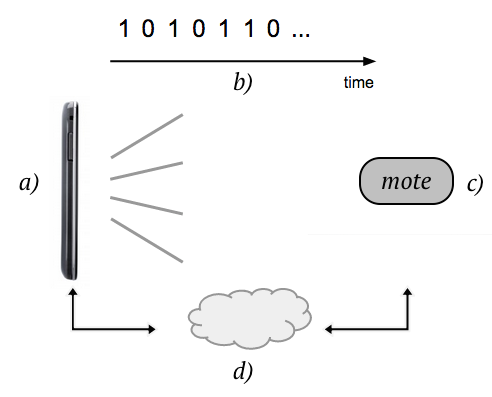
\includegraphics[scale=.4]{images/overview.png}
	\caption{Transmission of keying material with light: \textbf{a)} enter and encode key and parameters on smartphone, \textbf{b)} transmit them via light to the mote, \textbf{c)} persist key and parameters, \textbf{d)} communicate securely via the public Internet }
	\label{fig:overview}
\end{figure}

One method is to plug a wire to each and every node in order to initialize it.
However, there are two downsides: First, a typical IoT setup consists of too many devices for plugging to be a feasible solution. Second, in most installations, attackers may have physical access to motes, so jacks on the mote (e.g. JTAG) are a dangerous security threat.

Another approach is to pre-install the keys in the factory.
This would mean that either there is a small set of assigned keys, which would lead to possible brute-force attacks; or each mote gets an individual key, which requires a secure transmission and attribution of keys to motes\footnote{This would also increase cost of motes, but they need to be as cheap as possible in order to be affordable in great numbers.}.
Anyway, pre-initialization requires somebody other than the user/installer to know the keys, which diminishes security.

This paper proposes an alternative method, which is transmitting initial keying material via light.
Our method mainly targets private users without technical background.
As visible in Figure~\ref{fig:overview}, the user utilizes a smartphone application to enter, encode and emit keying material using the flash light of the phone.
The mote receives the message via a light sensor and reconstructs the keys.
After successful initialization and verification, the mote saves the keying material permanently.
On subsequent reboots, it is read from memory and immediately usable without any further action required.

There are several advantages of this method.
Light sensors are smaller and less misusable than jacks.
The physics of light is well understood by non-technical people, in contrast to radio waves.
Thus, leaking of the wirelessly sent secrets is less likely.
Moreover, multiple devices could be initialized concurrently by just placing them next to each other.

We implemented a prototype for an Android smartphone and a mote running the Contiki OS, \cite{dunkels04contiki}.
Contiki is an open source, state-of-the-art operating system for IoT devices\footnote{http://www.contiki-os.org/}.
We also tested techniques to make the transmission reliable.
Besides, we examined how fast the whole transmission could become while maintaining a high chance of correctness.

The remainder of the paper is structured as follows:
Section~\ref{sec:related_work} contains some background for security in the context of the~IoT and alternative approaches for key initialization.
In Section~\ref{sec:communication_protocol}, we propose our protocol for the smartphone and the mote to communicate via light.
Details of our implementations are presented in Section~\ref{sec:implementation}, both for the emitting~(Section~\ref{sub:android_app}) and the receiving~(Section~\ref{sub:mote}) parts.
In Section~\ref{sec:results_and_discussion}, we discuss our findings regarding the protocol and its limits.
In Section~\ref{sec:future_work}, we conclude our work and give suggestions for future research.


\section{Related Work}
\label{sec:related_work}

There are multiple approaches to key provisioning that secure the radio channel in some way, e.g.:

\cite{chen2011over} proposes key provisioning using eliptic curve cryptography (ECC).
However, while meeting high security standards, software implementations of ECC require a lot of memory and energy while hardware implementations increase the per-unit cost.
Moreover, they do not explain how public keys are provisioned.

In order to secure radio communication, \cite{kuo2007message} utilized a Faraday cage in which a batch of motes can be programmed without leaking messages to attackers outside of the cage.
Additionally, another device outside of the cage jams radio waves to prevent malicious communication.

\textit{6doku} is a protocol for pairing  a mote with a touch-enabled device like a smartphone, \cite{krentz20156doku}.
The smartphone needs extra hardware attached to communicate with the mote via radio waves.
It relies on interaction with the end-user as he needs to check if blinking on the screen happens in sync with him pressing a button on the mote.

There are also some proposals for key predistribution using an alternative channel, i.e. light:

\cite{saxena2009blink} proposes to generate public keys on the mote(s) and transfer them to a \textit{sink} via standard radio channels.
They are verified afterwards using the unidirectional light channel from the motes to the sink.
However, they still rely on energy consuming asymmetric encryption.

\textit{Light Communication for Deploying Secure Wireless Sensor Networks (LiDSN)} is an approach to assign a node id and a secret key to a mote, \cite{doan2012lidsn}.
Therefore, a temporal key for radio communication is transmitted to a specialized \textit{connector} via light.
The communication via light can be either way: if the connector receives light from the motes LED, it reads it. If the mote has no LED, a light sensor is assumed and the connector emits light with an own LED.
It is shown, that key provisioning is both faster and easier for end users.

\cite{electricimp} sells proprietary BlinkUp~\texttrademark  technology.
Instead of specialized hardware which end users might not want to buy, they provide a smartphone application which provisions a mote.
Assuming most users who install IoT setups already own a smartphone, this seems to be a cost-effective alternative.

However, we could not find that this approach is examined scientifically.
Thus, we propose a protocol for secure and wireless key predistribution using a smartphone as a light emitter and motes with a light sensor as receivers.

\section{Communication Protocol}
\label{sec:communication_protocol}

In the following section, we describe the phases of the protocol.
Each phase contains the necessary steps for the Android device and the mote.
Insights into the concrete implementation will be given in Section~\ref{sec:implementation}.

\subsection{Calibration}
\label{sub:calibration}

The goal of the calibration phase is to establish light values for \textit{bright} and \textit{dark} on the mote.
By doing this in the beginning of the protocol, we can adapt to different lighting situations in the room and different brightness levels of the phone.

The task of the phone in this protocol stage is simple.
It periodically sends \textit{bright} and \textit{dark} values, each with a certain period length $T$.
Simply said, it is blinking.

The mote on the other side measures $n$ light values using its light sensor.
The time between two measurements will probably not be equal to $T$, because the period length is unknown to the mote at this point.
As long as \textit{bright} and \textit{dark} values are part of the $n$ measurements, the concrete time does not matter.
After reading $n$ values, the mote calculates reasonable numeric values for \textit{bright} and \textit{dark}.
For instance, this can be achieved by applying a \mbox{\textit{2-means}} algorithm, see Section~\ref{ssub:contiki_process}.
After that, the mote is able to classify new light values and thus can read bits.

\subsection{Synchronization}
\label{sub:synchronization}

During synchronization, the mote learns the period length $T$.
This is necessary to be able to read light values at the right time (see Figure~\ref{fig:read_a_bit}).

In this phase, the phone keeps sending \textit{bright} and \textit{dark} values with the period length $T$.
This is the same as during calibration.

The mote on the other hand now measures light values as fast as it can and classifies them as \textit{0} and \textit{1}.
Once it notices that the bit flips, it records the time when the switch happened.
After recording $m$ bit flips, it can calculate the average period length.

With completion of the first two phases, the mote is now able to read data sent by the phone.
It learned a decision threshold for decoding the bits and the period length to read values at the right time.
Figure~\ref{fig:read_a_bit} shows how data can be read.
However, the actual implementation slightly differs from that figure, see Section~\ref{sec:implementation}.

\begin{figure}
	\centering
	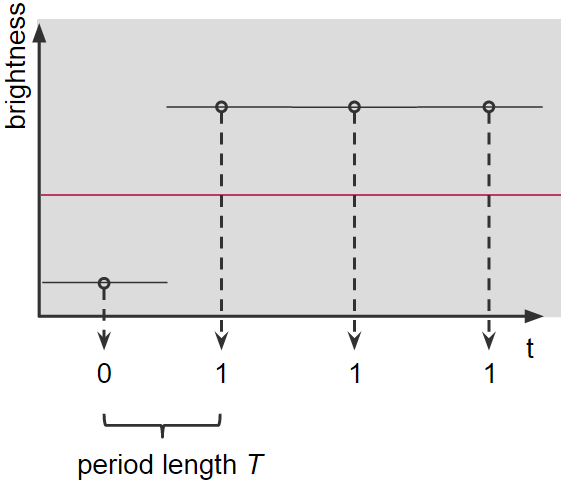
\includegraphics[scale=.5]{images/reading_data.png}
	\caption{Reading data: The black horizontal lines show the brightness emitted by the phone, the red line is the decision threshold for classifying \textit{0} and \textit{1}. Each arrow shows a point in time where the mote reads the value of the light sensor. The result here is the bit string 0111.}
	\label{fig:read_a_bit}
\end{figure}

\subsection{Initialization}
\label{sub:initialization}

The target of the initialization phase is to tell the mote when the actual data transmission starts.
The communication between the mote and the phone is one-way.
That means, the mote cannot communicate with the Android application.
Therefore, the application has to guess when the mote has successfully done calibration and synchronization.
This can either be done by using a fixed time (e.g. the application stays in calibration and synchronization phase for 10 seconds), or by user interaction (the user presses a button, when the mote indicates that it is ready via an LED).

When the phone reaches the initialization phase as a result of one of those methods, it sends a predefined initialization pattern.
The pattern must be different from $0101...$ and needs to have a length of one binary encoded character, e.g. 8~bit for ASCII encoding.
It sends the pattern exactly once, then it proceeds to the next phase.

After successful synchronization, the mote waits for the initialization pattern.
It does that by reading single bits and comparing the last 8~bits (for ASCII encoding) to the predefined pattern.
Once the initialization pattern has been detected, the mote immediately switches to the data sending phase.

\subsection{Data sending}
\label{sub:data_sending}

In the data sending phase, we can finally transmit the data packet.
As we can see in Figure~\ref{fig:data_packet}, the packet contains the data length, the actual data and a checksum used for validation of the received data in the validation phase~\ref{sub:validation}.

The Android application encodes the data string (e.g. ASCII encoding), measures its binary length and calculates the checksum using a predefined checksum algorithm.
It is obvious, that those calculations can be done beforehand.
The concatenated bit string then is sent using flashing of the display or the flash light.

The mote, after having recognized the initialization pattern, reads blocks of bits.
The first 4 byte are interpreted as the length of the actual data.
Afterwards, it reads the appropriate number of blocks to receive the data workload.
Once the whole data workload is read, it interprets the last 4 byte as the checksum.

\begin{figure}
	\centering
	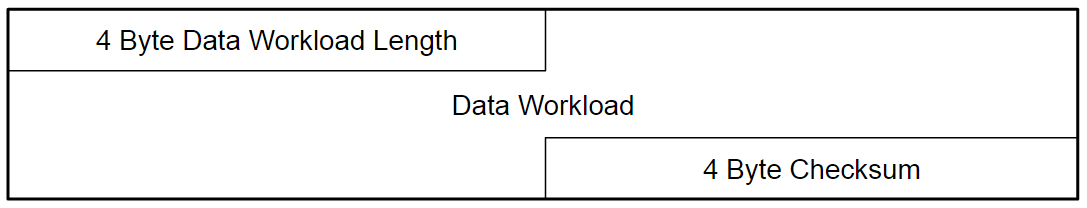
\includegraphics[scale=.3]{images/data_packet.png}
	\caption{Contents of the data packet: Besides the actual data, there is also the data length and a checksum transmitted.}
	\label{fig:data_packet}
\end{figure}

\subsection{Validation}
\label{sub:validation}

In this last phase, the mote checks whether the transmission was successful.
The phone does nothing in this phase, it has successfully run the protocol.
The mote uses the received data workload and calculates the checksum by itself.
If it is equal to the received one, the data packet is considered to be transmitted correctly.
If both checksums differ, something must have gone wrong.
It is not clear, whether the data workload was transmitted correctly and therefore the mote goes into an error state.

\section{Implementation}
\label{sec:implementation}

The implementation consists of an Android application\footnote{https://github.com/0x203/Flickerer/} that creates and sends the keying material and a Contiki process\footnote{https://github.com/Lixissimus/Security4Things} that runs on the TelosB sky mote and receives and validates it, \cite{dunkels04contiki}, \cite{telosb}.
Both follow the aforementioned communication protocol very closely, but increase reliability and fail-safeness through the following design decisions.

All data that is being sent is encoded with a \textit{Hamming(8,4)-code} so that two-bit errors can be detected and one-bit errors can be corrected.

The \textit{CRC32} is chosen as the checksum algorithm for the validation phase to avoid saving erroneous key material.
This could be caused by 3-or-more-bit errors that the Hamming code failed to detect.

As the Android timer that triggers the bit emission cannot be too early but in fact tends to be a little late\cite{mongia2010reliable}, the time at which the mote reads a bit is not in the middle of a period as suggested by Figure~\ref{fig:read_a_bit}.
It is at the very end of a period to maximize error avoidance due to timer delays\footnote{The Contiki timer that triggers the reading of the bit is a real-time timer.}.

In the following sections, both the implementation of the Android application and the Contiki process are described in more detail.

\subsection{Android app}
\label{sub:android_app}

We have developed two different versions of the Android application for users to enter keys and transmit them.

The first version is written using web technologies (i.e. HTML, CSS, and JavaScript) and deployed to the smartphone using Apache~Cordova\footnote{https://cordova.apache.org/}.
Because of this, the application can also run in most desktop browsers and can easily be ported to work with other smartphone operating systems, too, e.g. iOS or Windows Phone.
There are two disadvantages of this implementation, which motivated us to build a second edition:
The flash light cannot be controlled reliably using the mentioned web technologies.
This forced us to use the screen for light emission, which resulted in far smaller brightness margins to be read by the mote.
Furthermore the timing accuracy was considerably limited by the overhead caused by the Cordova runtime and the JavaScript interpreter which resulted in transmission errors.

\begin{figure}
	\centering
	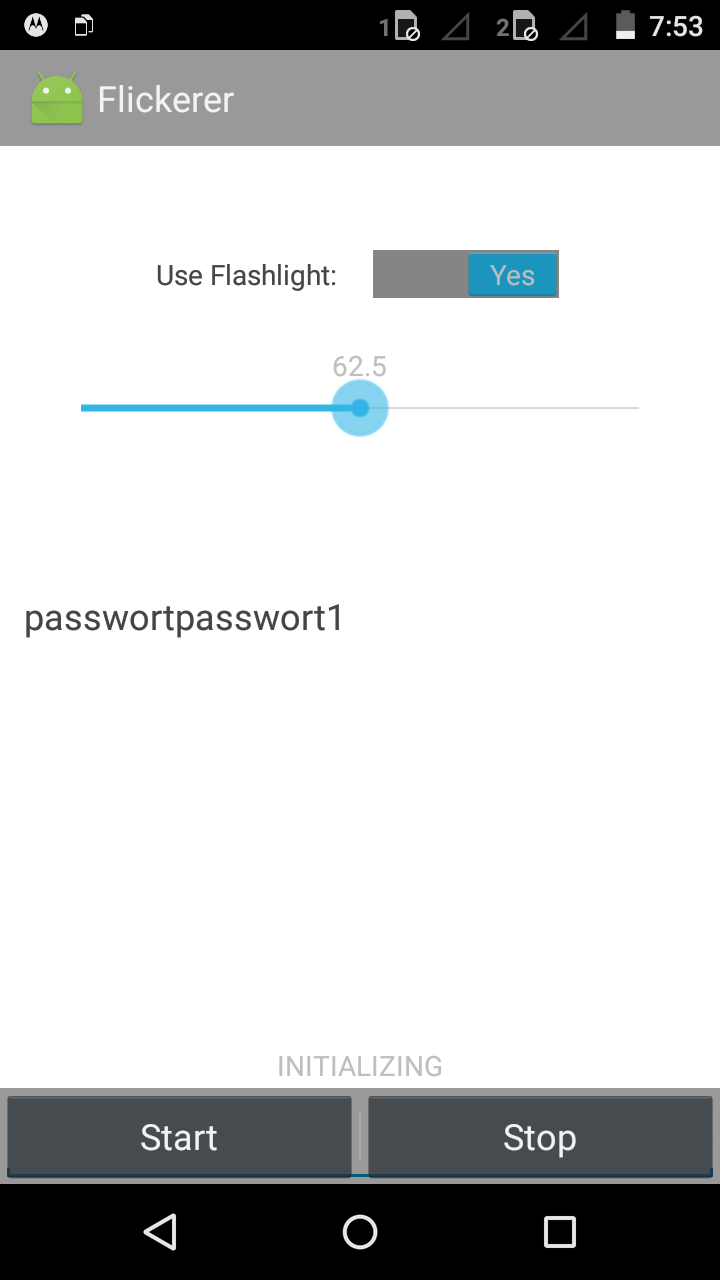
\includegraphics[scale=.15]{images/screen_native.png}
	\caption{Screenshot of the native Android application used to encode the key and emit it as light flickering. With a toggle switch the user can choose if the flashlight or the screen should flicker. The length of one bit can be adjusted using a slider. Any text entered in the text field can be transmitted by tapping on ``Start''. While transmitting, the user gets feedback about the current phase right above the buttons.}
	\label{fig:screenshot}
\end{figure}

To improve transmission reliability we therefore built a native Android application written in Java.
Still on Android, it is impossible to guarantee real-time behavior, but we may get smaller delays without JavaScript involved.
As to bee seen in Fig.~\ref{fig:screenshot}, any entered text will be ASCII-encoded and transmitted.
This is just a prove of concept, a real key should be a random 128~bit string which needs to be generated and saved for later usage, which is out of scope of this paper.
This Java implementation benefits from the ability of the native Java timer to re-adjust itself, which means that timing inaccuracies do not add up.
In that way, the phone and the mote do not get out of sync, no matter how long the transmission takes.
Another advantage of this version is the flash light.
Depending on the smartphone model, the flash light is as fast as screen flickering even for small bit lengths, while being much brighter.
Especially when attempting to program multiple motes at once this comes in very handy.


\subsection{Mote}
\label{sub:mote}

The implementation on the mote is divided into two parts.
The communication protocol and key storage is implemented in a Contiki process.
For the mote to securely communicate, the link layer needs to be initialized using the transmitted key, which is accomplished by a link layer driver wrapper.

\subsubsection{Contiki process}
\label{ssub:contiki_process}

The \textit{light process} implements the receiving side of the communication protocol.
A real-time timer called \textit{rtimer}, which is offered by the Contiki operating system, eliminates timer inaccuracies on the mote side.
The mote uses its light sensor to sense the current brightness.
Once the process is started, an LED-countdown (red $\rightarrow$ blue $\rightarrow$ green) indicates the start of the key initialization procedure.
A \mbox{\textit{2-means}} algorithm is used to create two clusters of \textit{bright} and \textit{dark} values and to compute their mean values~(see \ref{sub:calibration}).
Subsequently a new value is classified as \textit{0} or \textit{1} depending on which mean value is closer to it.
After the successful calibration, synchronization and initialization a blue LED indicates that the mote is receiving data.
If an error is detected by the Hamming-code or if the computed checksum does not match the transmitted one, a red LED indidcates the failure and the process should be restarted.
A green LED shows that the key material has been received successfully and was saved to the permanent flash memory of the mote.

\subsubsection{Contiki driver wrapper}
\label{ssub:contiki_driver_wrapper}

For the mote to actually use the key material that was transmitted, the initialization of the link layer security needs to be delayed until the key transmission finished successfully.
To do so we created a link layer driver wrapper that accomplishes the following things:

\begin{enumerate}
	\item Delay all calls to the link layer driver.
	\item Check whether the key material was initialized before.
	\item If not, start the \textit{light process} and wait for successful key transmission.
	\item Initialize the link layer using the transmitted key material.
	\item Forward all calls to the link layer driver.
\end{enumerate}

Calls to the driver that are being issued before the key material initialization are actually being canceled right now, but should eventually just be delayed and reissued once the initialization has finished.
Including the light app on a mote automatically redefines \textit{NETSTACK\_CONF\_LLSEC}\footnote{This global constant defines the link layer driver that is used by the mote.} to point to our link layer driver wrapper.
On the first start of the mote the key initialization via the \textit{light process} is triggered whereas during later starts the mote recognizes that its key material has been initialized before.


\section{Results and Discussion}
\label{sec:results_and_discussion}

Having a configurable transmission rate was very helpful during development and testing.
However it certainly introduces possible errors as the mote has to recognize the correct transmission rate, otherwise the initialization procedure will fail.
We decided against fixating it, as during our experiments the mote in all cases determined the correct transmission rate.
Also while testing different Android phones, we noticed each of it works best with a different transmission rate, so the app should change it depending on the phone model.

Figure~\ref{fig:successful_transmissions} shows the number of successful transmissions plotted against different transmission rates.
We used two different phones for measuring those values.
One is a \textit{Samsung Galaxy S2}, the other one is a \textit{Samsung Galaxy A3}.
As we can see, the \textit{A3} is able to send data at a considerabley higher transmission rate than the \textit{S2}.
While the \textit{A3} transmits reliably with a period length of 15ms, the \textit{S2} should not be used with a period length less than 62ms.
One reason for that could be that the \textit{A3} is considerably newer compared to the \textit{S2}.

We also tested the transmission reliability with a \textit{Motorola MotoG (2nd generation)} and an \textit{LG Nexus 5}.
Both showed very poor performance at arbitrary period lengths.
One possible explanation for this is, that the CPU of those phones is saving energy too aggressively.
This effect was already seen in \cite{mongia2010reliable}.
Different phone models seem to be affected differently by that.

\begin{figure}
	\centering
	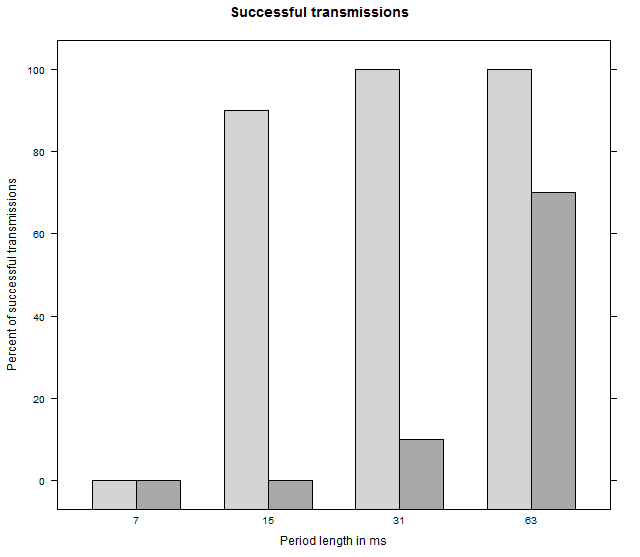
\includegraphics[scale=.35]{images/successful-transmissions.png}
	\caption{The light gray bars show the number of successful transmissions of the Samsung Galaxy A3, the dark gray bars the ones of the Samsung Galaxy S2. These are the results of 10 transmissions per period length. The transmitted string had a length of 16 characters and Hamming encoding was used.}
	\label{fig:successful_transmissions}
\end{figure}

Subject of debate is also the \textit{Hamming(8,4)-code}.
While it is able to correct one-bit-errors and detect two-bit-errors, it also doubles the amount of data to be sent.
When analyzing the number of corrected bits depending on the transmission rate, the following can be shown:
With long period lengths, the Hamming code does not detect or correct any errors, because the transmission happens without any errors.
When accelerating the transmission, there is a point where many bits are corrected, but the transmission normally succeeds.
If the transmission speed is then set even higher, the whole transmission fails most of the time due to irrecoverable errors.
The borders are 15ms for the \textit{A3} and 63ms for the \textit{S2} (see Figure~\ref{fig:successful_transmissions}).
When we want to achieve the transmission speed of the \textit{A3} with 15ms, we can either use the 15ms and Hamming encoding to correct the bits, or we can halve the amount of data by deactivating the Hamming encoding and transmit with 31ms per bit\footnote{The values are rounded, that is why the half of 31 is 15.}.
So the transmission takes the same time, but actually increases the percentage of successful transmissions.
Errors can still be detected afterwards using the \textit{CRC32} checksum.
Therefore, the \textit{Hamming(8,4)-code} is not useful in that case.



\section{Conclusion and Future Work}
\label{sec:future_work}

In this paper, we presented a secure method for IoT-device initialization by transmitting initial keying material via light.
It is mainly targeted at private users and can easily be executed having no technical background at all.
As the visibility of light can be judged and restricted pretty well by end users, safety from interception is given.

Future work should target the further automation of the presented process, e.g. by establishing a bidirectional communication.
Using its camera the mobile phone could detect the current LED-state of the mote and react accordingly, e.g. start the data transmission or restart the whole process.

To simplify the initialization of several motes at once, two things need to be done.
First, the Android application should stay in calibration and synchronization phase, until the user presses a button.
Second, the mote should indicate via an LED that it reached the initialization phase~(see \ref{sub:initialization}).
With those two concepts, the key transmission to several motes could work as follows:
The user lays out all motes in a grid next to each other.
Then the phone is placed on top of them and the app is started.
All motes are placed, so that they receive the flickering of the flash light.
The motes are started one after another.
Once the motes are running, the user waits for all of them to indicate via an LED, that they reached the initialization phase.
They are now all waiting for the initialization pattern.
The user presses a button in the application and the phone sends the initialization pattern followed by the data packet.
When the transmission is over, the user can see via a red LED which motes failed to receive the data correctly.
The process needs to be restarted with those motes.
However, this is not implemented and tested yet and could be part of future projects.

% Bibliography
% \bibliographystyle{ACM-Reference-Format-Journals}
\bibliographystyle{abbrv}
\bibliography{paper}

\end{document}
